\chapter{Metodología}\label{ch:metodologia}
%  VISIÓN GENERAL DEL CAPÍTULO
La metodología caracteriza la distribución espacial y la magnitud de los máximos de precipitación y viento asociados a los ciclones extratropicales del Atlántico Sur, mediante un marco de referencia lagrangiano centrado en el sistema y condicionado por la fase del ciclo de vida y la región de ciclogénesis.
La estrategia sigue cinco etapas: (1) definición de las fuentes de datos; (2) construcción y estratificación de las poblaciones de ciclones; (3) procesamiento lagrangiano de los campos de superficie; (4) caracterización estadística univariada mediante estimación de densidad y análisis EOF; y (5) análisis multivariado (MEOF) y construcción de prototipos estructurales.
Los prototipos se organizan en $3 \times 4$ paneles (3 regiones de ciclogénesis $\times$ 4 fases evolutivas) para la Población Global (PG) y el subconjunto p90.

%  SECCIÓN M1 — DATOS
\section{Datos}\label{sec:datos}

\subsection{Reanálisis ERA5}\label{sec:datos_era5}

Se utiliza el reanálisis de quinta generación del ECMWF, ERA5 \citep{hersbach2020era5}, mediante el conjunto de datos \textit{``ERA5 hourly data on single levels from 1940 to present''} \citep{hersbach_era5_2023b} para el período 1979--2020.
La justificación de ERA5, resolución espacial ($\sim$31 km) y temporal (horaria), y su mayor densidad de trayectorias y representación de estructuras de mesoescala frente a reanálisis previos \citep{gramcianinov2020analysis}, es la base de la elección de este reanálisis para el catálogo de trayectorias.
No obstante, \citet{chen2024evaluation} demuestran que ERA5 subestima sistemáticamente los extremos del 5\% de ciclones extratropicales más intensos, con sesgos del $-10.2\%$ en viento y $-22.6\%$ en precipitación respecto a observaciones en Estados Unidos de América.
Por ello, los resultados obtenidos para p90 deben interpretarse como estimaciones conservadoras de la intensidad real de los eventos.

\subsection{Variables meteorológicas}\label{subsec:variables}

El análisis se realiza a partir de campos horarios de ERA5, con las siguientes variables de superficie:

\begin{itemize}
    \item Precipitación total acumulada (\texttt{tp}, en mm\,h$^{-1}$).
    \item Magnitud del viento en superficie a 10 m (\texttt{wind10}, en m\,s$^{-1}$).
\end{itemize}

La elección de ambas variables responde a la naturaleza morfológica de los ciclones extratropicales y a la estructura de sus campos de precipitación y viento, fundamentada en la Sección~\ref{subsec:tb_compound_def} de los Fundamentos.
Este enfoque describe la configuración espacial típica de los campos de superficie en cada fase evolutiva y permite evaluar la eventual co-ocurrencia de los máximos de ambas variables, como primer acercamiento al análisis multivariado (MEOF) detallado en la Sección~\ref{subsec:eof_multivariado}.

\subsection{Base de trayectorias y fases}\label{sec:bd_ciclones}
El punto de partida es el catálogo de trayectorias desarrollado por \citet{gramcianinov2020analysis} a partir de ERA5, cuya alta resolución permite capturar sistemas de mesoescala y ciclogénesis en la región de estudio.
Los parámetros del algoritmo de seguimiento y los filtros aplicados se detallan en la Tabla~\ref{tab:tracking_params}.

\begin{table}[ht]
\centering
\caption[Parámetros y filtros de la base de trayectorias]{Parámetros técnicos y filtros aplicados en la base de datos de trayectorias \citep{gramcianinov2020analysis}.}
\label{tab:tracking_params}
\begin{tabular*}{\textwidth}{@{\extracolsep{\fill}}ll}
\hline
Parámetro & Especificación \\ 
\hline
Fuente de datos & ERA5 (ECMWF) \\
Resolución espacial & $\sim$31 km ($0.25^\circ \times 0.25^\circ$) \\
Variable de seguimiento & Vorticidad relativa en 850 hPa ($\zeta_{850}$) \\
% % Nivel de filtrado espectral & T42 (para aislar la escala sinóptica) \\
% % Umbral de intensidad & $\zeta_{850} < -1.0 \times 10^{-5}$ s$^{-1}$ \\
Duración mínima & 24 horas \\
Desplazamiento mínimo & 1000 km \\ 
\hline
\end{tabular*}
\end{table}

% \begin{table}[ht]
% \centering
% \caption{Parámetros técnicos y filtros aplicados en la base de datos de trayectorias \citep{gramcianinov2019properties}.}
% \label{tab:tracking_params}
% \begin{tabular*}{\textwidth}{@{\extracolsep{\fill}}ll}
% \hline
% Parámetro & Especificación \\ 
% \hline
% Fuente de datos & ERA5 (ECMWF) \\
% Resolución espacial & $\sim$31 km ($0.25^\circ \times 0.25^\circ$) \\
% Variable de seguimiento & Vorticidad relativa en 850 hPa ($\zeta_{850}$) \\
% % % Nivel de filtrado espectral & T42 (para aislar la escala sinóptica) \\
% % % Umbral de intensidad & $\zeta_{850} < -1.0 \times 10^{-5}$ s$^{-1}$ \\
% Duración mínima & 24 horas \\
% Desplazamiento mínimo & 1000 km \\ 
% \hline
% \end{tabular*}
% \end{table}


Sobre esta base, \citet{coutodesouza2024new} incorporan una clasificación objetiva de las fases evolutivas mediante el algoritmo \textit{CycloPhaser} \citep{deSouza2025CycloPhaser}, que evalúa la tasa de cambio de la vorticidad relativa en 850 hPa ($\zeta_{850}$) para segmentar matemáticamente el desarrollo y decaimiento de cada sistema.
Los fundamentos físicos de esta elección de $\zeta_{850}$ y de la segmentación en cuatro fases se exponen en las Secciones~\ref{subsec:tb_zeta} y~\ref{subsec:tb_fases} de los Fundamentos. La Tabla~\ref{tab:fases_def} resume dichas fases.

\input{tabelas_es/tab_fases_def.tex}

%  SECCIÓN M2 — POBLACIONES DE ESTUDIO

\section{Construcción de las poblaciones de estudio}\label{sec:poblaciones_estudio}

La segmentación de la muestra sigue los criterios de la Sección~\ref{subsec:tb_poblaciones} de los Fundamentos.
La base de trayectorias se divide en una población de referencia y, a partir de ella, un subconjunto de alta intensidad ($p90$).
Ambas poblaciones se construyen de forma independiente para cada una de las tres regiones de ciclogénesis (SBR, LPB y ARG), delimitadas según la taxonomía de \citet{gramcianinov2019properties} y detalladas en la Tabla~\ref{tab:regiones_coords}.
Esta estratificación geográfica responde a que las regiones presentan regímenes dinámicos diferenciados, discutidos en la Sección~\ref{sec:tb_regiones} de los Fundamentos.

\input{tabelas_es/tab_regiones_coords.tex}

\subsection{Población Global (PG): referencia}\label{subsec:grupo_global}

La Población Global establece el comportamiento morfológico y estadístico medio de los ciclones con desarrollo típico y completo en la región.
Se aplica un criterio de coherencia evolutiva, seleccionando únicamente los sistemas que cumplieron dos criterios simultáneos:

\begin{enumerate}
    \item Ciclo de vida completo: Presencia confirmada y secuencial de las cuatro fases de desarrollo, incipiente (\textit{incipient}), intensificación (\textit{intensification}), madurez (\textit{mature}) y decaimiento (\textit{decay}).
    \item Ausencia de fases complejas: Exclusión categórica de sistemas que desarrollaron fases secundarias, de re-intensificación (p. ej., \textit{intensification~2}, \textit{mature~2}) o fases residuales (\textit{residual}).
\end{enumerate}

Esto elimina el ruido de sistemas efímeros o de evolución errática.
Para cada ciclón de la PG se identifica el registro temporal de su máxima intensidad, el extremo absoluto de vorticidad relativa a 850 hPa, $\zeta_{850}^{\min}$, como métrica de intensidad para la extracción posterior del subconjunto p90.

La Figura~\ref{fig:loc_vort_global} sintetiza la densidad de probabilidad de la ubicación donde los ciclones de la PG alcanzan su $\zeta_{850}^{\min}$ a lo largo de su ciclo de vida, con el número de ciclones detallado en la Tabla~\ref{tab:conteo_ciclones}.

\begin{figure}[htbp]
\centering
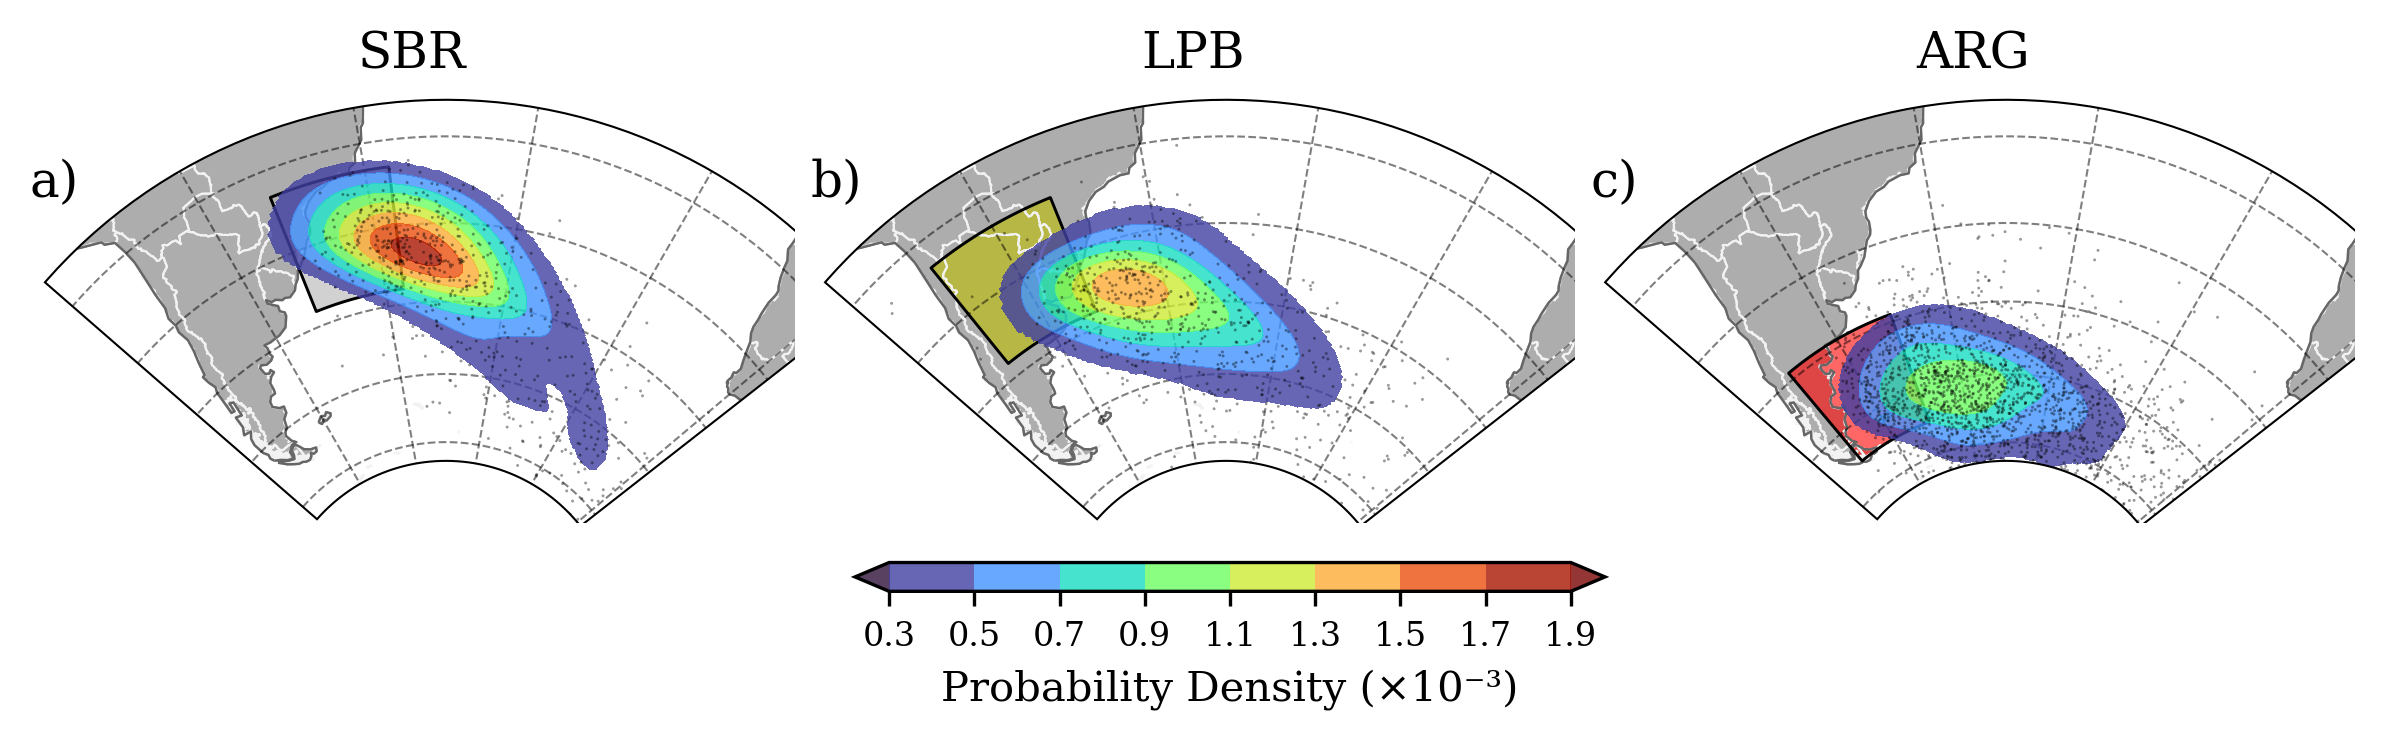
\includegraphics[width=\textwidth]{images/geral/vort_global_vf.png}
\caption[Ubicación del mínimo de vorticidad (Población Global)]{Distribución espacial de la densidad de probabilidad de la ubicación donde los ciclones de la PG alcanzan su menor vorticidad relativa a 850~hPa ($\zeta_{850}^{\min}$) a lo largo de su ciclo de vida. a), b), y c) corresponden a las regiones de ciclogénesis SBR, LPB y ARG, respectivamente. Los contornos de colores indican la densidad de probabilidad ($\times 10^{-3}$) y los puntos grises marcan las posiciones individuales de los mínimos.}
\label{fig:loc_vort_global}
\end{figure}


\subsection{Subconjunto de alta intensidad (p90)}\label{subsec:subconjuntos_intensidad}

Para evaluar los patrones espaciales frente a la severidad dinámica del sistema, se extrae de la PG el 10\% de ciclones con los valores más negativos de $\zeta_{850}^{\min}$ (un decil de la distribución), obteniendo el subconjunto $p90$ (detallado en \ref{subsec:tb_poblaciones}).

La Tabla~\ref{tab:conteo_ciclones} documenta la reducción del tamaño muestral desde la base cruda hasta la PG y el subconjunto p90.

\input{tabelas_es/tab_conteo_ciclones.tex}

El análisis de la fase en que se registra el pico de vorticidad (Tabla~\ref{tab:fase_max_intensidad}) confirma que p90 respeta la estructura dinámica dominante. Cerca del 83\% de los casos alcanza su mínima intensidad durante la fase de madurez, frente a menos del 5\% durante el decaimiento.

\input{tabelas_es/tab_fase_max_intensidad.tex}

La Figura~\ref{fig:loc_vort_p90} muestra la distribución espacial de la densidad de probabilidad de la ubicación del mínimo de vorticidad del subconjunto p90.

% Figura para el subconjunto p90 (Subsección 2)
\begin{figure}[htbp]
\centering
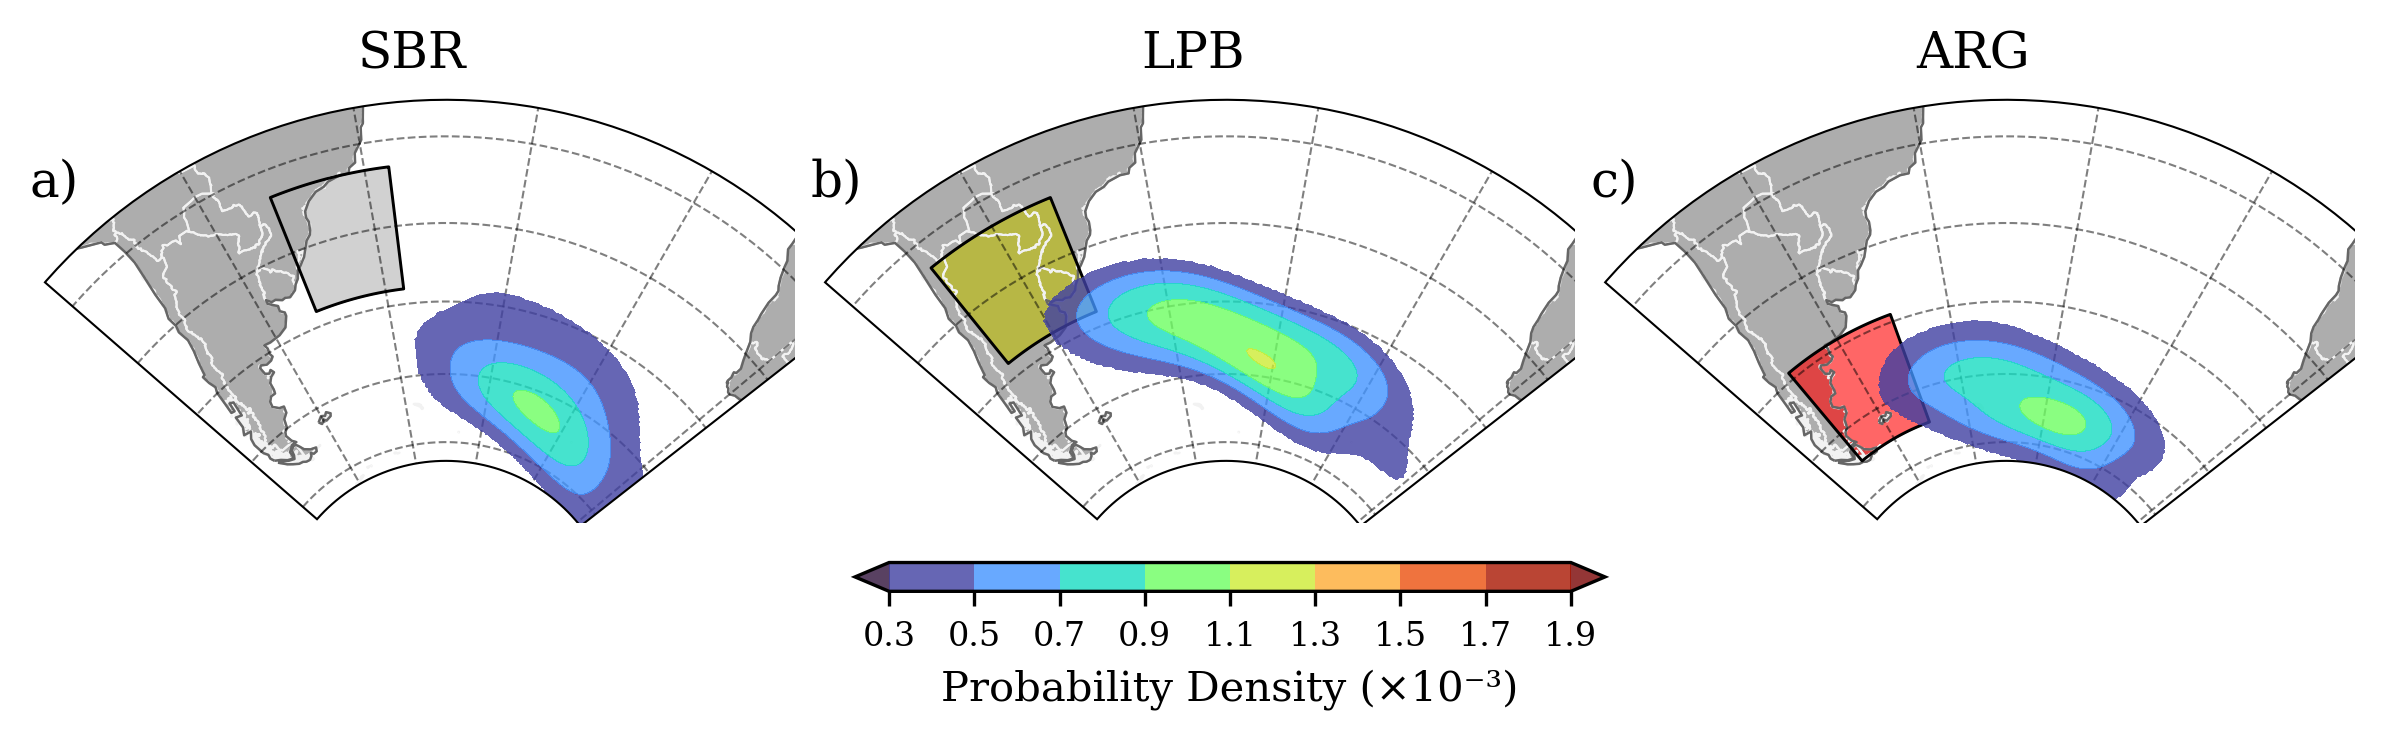
\includegraphics[width=\textwidth]{images/geral/vort_p90_vf.png}
\caption[Ubicación del mínimo de vorticidad (subconjunto p90)]{Similar a la Figura~\ref{fig:loc_vort_global} pero para el subconjunto p90 (sistemas más intensos, decil inferior de $\zeta_{850}^{\min}$).}
\label{fig:loc_vort_p90}
\end{figure}

Sobre el subconjunto p90, comparándolo sistemáticamente con la PG, se aplica íntegramente el flujo metodológico descrito en las secciones siguientes para evaluar si una mayor intensidad dinámica del vórtice se asocia con cambios en: (i) la magnitud absoluta de los máximos de viento y precipitación; (ii) la distribución espacial relativa de dichos máximos; y (iii) los patrones estructurales dominantes identificados por el MEOF.

% ============================================================
%  SECCIÓN M3 — PROCESAMIENTO LAGRANGIANO
% ============================================================

\section{Procesamiento lagrangiano}\label{sec:procesamiento_lagrangiano}

Para caracterizar la estructura de los sistemas independientemente de su ubicación geográfica, se adopta el marco lagrangiano expuesto en la Sección~\ref{subsec:tb_lagrangiano} de los Fundamentos, un dominio móvil de $20^{\circ} \times 20^{\circ}$ centrado en la posición del mínimo de vorticidad para cada instante $t$ de la trayectoria, en coordenadas relativas $(\Delta x, \Delta y)$ respecto al núcleo ciclónico. Este dominio aísla la señal de mesoescala y representa físicamente la extensión espacial de los brazos frontales del sistema. El procesamiento se realiza por separado para cada combinación de región de ciclogénesis y fase del ciclo de vida.

Siguiendo la técnica de compositing centrado en el sistema (Sección~\ref{subsubsec:tb_compositing}), y para reducir la variabilidad de alta frecuencia de los datos horarios y aislar la condición estructural más representativa de cada fase, se aplica un promediado centrado. Para cada ciclón y fase se seleccionan los registros horarios del núcleo temporal de la fase, dos tiempos cuando el número de horas es par, tres cuando es impar, y se promedian sus campos espaciales. Así, el campo resultante refleja la condición arquetípica del régimen (incipiente, intensificación, madurez o decaimiento) y no una mezcla de dos estados sucesivos, generando un único campo promedio por ciclón--fase que constituye la unidad de análisis de todas las etapas estadísticas subsiguientes. En consecuencia, cada ciclón aporta un campo independiente a cada una de las cuatro poblaciones fase-específicas de su región, de modo que el tamaño muestral $m$ de los análisis estadísticos de las secciones siguientes es constante entre fases dentro de una misma región e igual al número de ciclones reportado en la Tabla~\ref{tab:conteo_ciclones}.

% ============================================================
%  SECCIÓN M4 — CARACTERIZACIÓN ESTADÍSTICA UNIVARIADA
% ============================================================

\section{Caracterización estadística univariada}\label{sec:tecnicas_estadisticas}

\subsection{Extracción de máximos y distribución de probabilidad (PDF)}\label{subsec:extraccion_pdf}

Sobre el campo promedio por ciclón--fase se aplica un suavizado espacial bidimensional con filtro gaussiano ($\sigma = 0.25$, biblioteca \texttt{scipy}) para evitar valores aislados a escala de punto de grilla. Luego se delimita el área de análisis con una máscara circular de $9.5^{\circ}$ de radio centrada en el núcleo del sistema, inscrita en el dominio lagrangiano de $20^{\circ} \times 20^{\circ}$, de modo que una franja perimetral de $0.5^{\circ}$ en cada borde queda excluida. Dentro de este radio se identifican: (i) la magnitud del valor máximo absoluto de la variable de interés, $x_i$, y (ii) su ubicación en coordenadas relativas al centro del ciclón, $\mathbf{s}_i = (\Delta x_i, \Delta y_i)$. El procedimiento genera, para cada combinación de región, fase evolutiva y variable, un conjunto de $m$ pares magnitud--ubicación (uno por evento ciclónico).

Para caracterizar la distribución de las magnitudes máximas extraídas $\{x_i\}_{i=1}^{m}$ se estima la función de densidad de probabilidad (PDF) mediante KDE; su justificación frente a histogramas y su formulación matemática se presentan en la Sección~\ref{subsubsec:tb_kde} de los Fundamentos. La implementación usa la clase \texttt{gaussian\_kde} de \texttt{scipy.stats}, con ancho de banda $h$ según la regla de Scott \ref{eq:tb_kde_pdf} y el núcleo gaussiano de la Ecuación~\ref{eq:tb_gaussian_kernel} de los Fundamentos. Las curvas PDF permiten contrastar cuantitativamente cómo evolucionan las magnitudes a lo largo del ciclo de vida y cómo difieren entre la PG y p90.

\subsection{Distribución espacial de los máximos}\label{subsec:kde_localizacion}

Para caracterizar la ubicación preferencial de los máximos respecto al centro del ciclón, la posición relativa de cada máximo se trata como variable aleatoria bidimensional $\mathbf{S} = (\Delta x, \Delta y)$. A partir del conjunto de $m$ ubicaciones relativas $\{\mathbf{s}_i\}_{i=1}^{m}$ de la etapa anterior, se estima la función de densidad de probabilidad de la posición (PDFe), $\hat{f}(\mathbf{s})$, mediante el estimador kernel bidimensional de la Sección~\ref{subsubsec:tb_kde} (Ecuaciones~\ref{eq:tb_kde_simple}--\ref{eq:tb_gauss_kernel_2d_simple}).

A diferencia de la PDF de magnitudes (Sección~\ref{subsec:extraccion_pdf}), la PDFe cuantifica la densidad de probabilidad de que el máximo ocurra en una posición relativa dada $\mathbf{s} = (\Delta x, \Delta y)$, independientemente del valor numérico de precipitación o viento en ese punto. El resultado es un campo continuo de densidad de probabilidad sobre el dominio centrado.

\subsection{Análisis de Funciones Ortogonales Empíricas (EOF) univariado}\label{subsec:eof_univariado}

Para identificar los patrones espaciales dominantes de variabilidad estructural se aplica un análisis EOF sobre el conjunto de $m$ campos promedio por ciclón--fase, por separado para cada variable (precipitación, viento), región y fase. Las referencias previas de este enfoque se presentaron en la Sección~\ref{subsubsec:tb_eof}. Previo al análisis, a cada campo se le resta la media del ensamble en cada punto de grilla para obtener las anomalías estructurales:

\begin{equation}
    X'(\tau, \mathbf{s}) = X(\tau, \mathbf{s}) - \frac{1}{m}\sum_{\tau=1}^{m}X(\tau, \mathbf{s}),
\end{equation}

donde $X(\tau, \mathbf{s})$ es el campo de la variable para el ciclón $\tau$ en la posición relativa $\mathbf{s} = (x,y)$. De la matriz de anomalías se calcula la matriz de covarianza espacial, cuya diagonalización produce los modos ortogonales ($\text{EOF}_k$) y sus amplitudes ($\text{PC}_k$):

\begin{equation}
    X'(\tau, \mathbf{s}) = \sum_{k=1}^{K} \text{PC}_k(\tau) \cdot \text{EOF}_k(\mathbf{s}).
\end{equation}

No se aplica remoción de tendencia temporal (\textit{detrend}). El eje muestral es un índice de eventos discretos con espaciado temporal irregular entre 1979--2020, por lo que un ajuste lineal cronológico asumiría erróneamente un espaciado constante. El objetivo físico es aislar las características morfológicas de la variabilidad inter-sistémica dentro de cada fase, no las tendencias climáticas de baja frecuencia. La implementación utiliza la biblioteca \texttt{xeofs} \citep{rieger2024xeofs} sobre estructuras \texttt{xarray}.

Cabe señalar que el tamaño muestral $m$ difiere sustancialmente entre regiones (Tabla~\ref{tab:conteo_ciclones}). ARG cuenta con la muestra más numerosa (1980 en la PG, 198 en p90), mientras que SBR y LPB presentan muestras considerablemente menores (641/64 y 669/67, respectivamente). Esta asimetría implica que los autovectores de SBR y LPB están sujetos a mayor incertidumbre de muestreo que los de ARG, lo que motiva la evaluación de significancia estadística mediante Bootstrap-t descrita en la Sección~\ref{subsec:bootstrap_significancia}.

\subsection{Significancia espacial: Bootstrap-t}\label{subsec:bootstrap_significancia}

Para evaluar la robustez estadística de los autovectores del EOF y aislar las señales físicas del ruido estocástico, se implementa el remuestreo no paramétrico Bootstrap-t; su elección y ventajas frente al Bootstrap percentílico estándar para distribuciones asimétricas y de cola pesada se fundamentaron en la Sección~\ref{subsubsec:tb_bootstrap} de los Fundamentos. Se generan $R = 15{,}000$ submuestras con reemplazo, garantizando error de Monte Carlo insignificante en la estimación de las colas de la distribución.

Para cada iteración $b$ se recalcula el EOF sobre la submuestra y, en cada punto de grilla, se obtiene el estadístico cuasi-pivotal:

\begin{equation}
    t^*_b(\mathbf{s}) = \frac{\hat{\theta}^*_b(\mathbf{s}) - \hat{\theta}(\mathbf{s})}{SE^*_b(\mathbf{s})},
\end{equation}

donde $\hat{\theta}(\mathbf{s})$ es la carga espacial original en $\mathbf{s}$, $\hat{\theta}^*_b(\mathbf{s})$ su estimación en la submuestra y $SE^*_b(\mathbf{s})$ su error estándar estimado. Los intervalos de confianza al 95\% se obtienen invirtiendo los cuantiles empíricos $q_{\alpha/2}$ y $q_{1-\alpha/2}$ de la distribución de $t^*$ (con $\alpha = 0.05$):

\begin{equation}
    \left(\hat{\theta}(\mathbf{s}) - q_{1-\alpha/2}\,SE(\mathbf{s}),\; \hat{\theta}(\mathbf{s}) - q_{\alpha/2}\,SE(\mathbf{s})\right).
\end{equation}

Los puntos de grilla se consideran estadísticamente significativos si su intervalo de confianza excluye el cero.

\subsection{Análisis de las Componentes Principales (PC1)}\label{subsec:analisis_pc}

Además de la descomposición espacial, se analizan las propiedades estadísticas de la Componente Principal del primer modo (PC1), que representa la amplitud de cada ciclón sobre el patrón estructural dominante; la interpretación cualitativa de estos momentos estadísticos se estableció en la Sección~\ref{subsubsec:tb_eof} de los Fundamentos. Se calculan, para la serie de PC1 de cada variable, región y fase, la asimetría ($\gamma_1$):
\begin{equation}
    \gamma_1 = \frac{1}{m} \sum_{\tau=1}^{m} \left(\frac{PC_{1,\tau} - \overline{PC_1}}{\sigma_{PC_1}}\right)^3,
\end{equation}
y la curtosis ($\gamma_2$):
\begin{equation}
    \gamma_2 = \frac{1}{m} \sum_{\tau=1}^{m} \left(\frac{PC_{1,\tau} - \overline{PC_1}}{\sigma_{PC_1}}\right)^4 - 3.
\end{equation}
Para conectar físicamente la estructura de los campos de superficie con la intensidad del sistema, se evalúa la correlación de Pearson entre la PC1 de cada variable y el mínimo de vorticidad relativa $\zeta_{850}^{\min}$ (negativa en el Hemisferio Sur):
\begin{equation}
    \rho\!\left(PC_1, \zeta_{850}^{\min}\right) = \frac{\text{cov}\!\left(PC_1, \zeta_{850}^{\min}\right)}{\sigma_{PC_1} \cdot \sigma_{\zeta}}.
\end{equation}
Su interpretación físico-estadística, el vínculo entre la proyección sobre el modo dominante y la intensidad dinámica del sistema, se estableció en la Sección~\ref{subsubsec:tb_eof} de los Fundamentos.

Para evaluar si los patrones dominantes de precipitación y viento varían conjuntamente, se calcula la correlación entre las PC1 de precipitación y viento dentro de cada región y fase:
\begin{equation}
    \rho = \text{corr}\!\left(PC_1^{\text{precip}},\; PC_1^{\text{viento}}\right).
\end{equation}
Valores cercanos a $+1$ indican que precipitación y viento se organizan espacialmente de manera coherente; valores cercanos a $0$ sugieren que la variabilidad espacial de la precipitación está controlada por procesos locales independientes de la configuración de mayor escala.

% ============================================================
%  SECCIÓN M5 — ANÁLISIS MULTIVARIADO Y PROTOTIPOS
% ============================================================

\section{Análisis multivariado y prototipos estructurales}\label{sec:meof_prototipos}

\subsection{EOF combinado (MEOF) precipitación--viento}\label{subsec:eof_multivariado}

Para identificar los patrones espaciales dominantes de la estructura combinada de precipitación y viento se realiza un análisis EOF combinado (MEOF). A diferencia del análisis univariado, el MEOF captura modos de variabilidad conjunta que reflejan la organización morfológica típica de los campos de superficie asociados a la dinámica ciclónica. Los fundamentos de esta técnica, incluyendo la necesidad de normalizar variables con unidades físicas dispares y la lógica de la concatenación espacial del vector de estado, se expusieron en la Sección~\ref{subsubsec:tb_eof} de los Fundamentos. Aunque el MEOF es habitual en estudios de eventos simultáneos, aquí se emplea exclusivamente como herramienta de síntesis estructural, para aislar las configuraciones espaciales más recurrentes de los campos de superficie. El procedimiento consta de tres pasos:

\paragraph{Paso 1 — Anomalías.} Se calcula el campo de anomalías de cada variable respecto a la media del conjunto (PG o p90) en cada punto de grilla.

\paragraph{Paso 2 — Normalización por desviación estándar espacialmente promediada.} Para preservar los gradientes espaciales nativos de cada campo, la normalización usa un escalar global único por variable:
\begin{equation}
    Z_{V}(\tau, \mathbf{s}) =
        \frac{V'(\tau, \mathbf{s})}{\bar{\sigma}_{V}},
    \qquad
    \bar{\sigma}_{V} = \frac{1}{N_s} \sum_{i=1}^{N_s} \sigma_{V}(\mathbf{s}_i),
\end{equation}
donde $V'$ es el campo de anomalías, $\sigma_{V}(\mathbf{s}_i)$ la desviación estándar temporal en el punto de grilla $\mathbf{s}_i$, y $N_s$ el número total de puntos de grilla del dominio. La media se calcula como promedio aritmético simple de los puntos de grilla.
Este factor escalar preserva la estructura espacial de los gradientes mientras equilibra el peso de ambas variables en la matriz de covarianza, evitando que el campo de mayor varianza domine artificialmente la descomposición conjunta \citep{wilks2019statistical_ch13}.

\paragraph{Paso 3 — Concatenación espacial.} Los campos normalizados se concatenan para formar el vector de estado combinado:

\begin{equation}\label{eq:meof_vector}
    \mathbf{Y}(\tau) = \big[ Z_P(\tau),\; Z_W(\tau) \big].
\end{equation}

El EOF aplicado a la matriz combinada $\mathbf{Y}(\tau)$ produce modos acoplados que explican la varianza conjunta del sistema. El MEOF$_1$ produce simultáneamente un patrón espacial para precipitación ($\text{EOF}_{1,P}$) y otro para viento ($\text{EOF}_{1,W}$), ambos extraídos del mismo modo dominante de covariabilidad conjunta.

Tanto la PG como el subconjunto p90 se procesan de forma independiente con este mismo procedimiento, de modo que los patrones estructurales resultan exclusivamente de su propia covarianza interna.

\subsection{Construcción de los prototipos estructurales}\label{subsec:prototipos}

Para cumplir con el Objetivo Específico 4, se desarrolla un procedimiento de síntesis visual que integra en un único panel, por cada combinación región-fase, cuatro fuentes de información estadística derivadas de los análisis anteriores. Cada prototipo se compone de cuatro capas superpuestas en coordenadas lagrangianas $(\Delta x, \Delta y)$, dentro del dominio de $9.5^{\circ}$ de radio. La lógica del compositing centrado en el sistema, que hace posible esta superposición, se presentó en la Sección~\ref{subsubsec:tb_compositing} de los Fundamentos.

Las dos primeras capas son las isolíneas de la PDFe de la ubicación de máximos de precipitación y viento. A partir de la superficie de densidad $\hat{f}(\mathbf{s})$ (Ecuación~\ref{eq:tb_kde_simple}) se extraen los contornos de los percentiles 75 y 90 de la densidad acumulada, y sobre cada superficie se señaliza con un marcador estelar la coordenada $(\Delta x_{\text{moda}}, \Delta y_{\text{moda}})$, la posición donde es más frecuente encontrar el máximo de la variable.

Las capas tercera y cuarta muestran las isolíneas de los patrones espaciales del primer modo multivariado (MEOF$_1$), obtenidos según la Sección~\ref{subsec:eof_multivariado} para precipitación ($\text{EOF}_{1,P}$) y viento ($\text{EOF}_{1,W}$).
Previo al trazado de contornos se aplica un suavizado gaussiano ($\sigma = 2$) a cada campo. Los niveles de contorno se determinan mediante percentiles aplicados por separado sobre los valores positivos (percentiles 33 y 66, línea sólida) y negativos (percentiles 33 y 66 del valor absoluto, línea discontinua).
Esta umbralización relativa garantiza comparabilidad entre distintas combinaciones región--fase, independientemente de la magnitud absoluta del patrón espacial del MEOF.
Las regiones de carga positiva indican sectores donde la variable tiende a presentar anomalías positivas respecto a la media cuando el modo dominante se activa; las de carga negativa, supresión relativa.

El resultado se organiza en una figura matricial de $3 \times 4$ paneles (3 regiones de ciclogénesis $\times$ 4 fases evolutivas), donde cada panel integra las cuatro capas descritas: PDFe de precipitación, PDFe de viento, $\text{EOF}_{1,P}$ de precipitación y $\text{EOF}_{1,W}$ de viento.
La superposición permite identificar el grado de organización espacial entre ambos campos en el entorno del ciclón.
Una alta coincidencia entre el núcleo del PDFe de precipitación y la región de carga positiva del EOF de viento indica una estructura frontal compacta; un desacoplamiento revela asimetrías en la distribución de los máximos, posiblemente asociadas a procesos locales de interacción océano-atmósfera o a la geometría del frente.
Este análisis ofrece, además, un marco de referencia para detectar configuraciones que podrían favorecer eventos simultáneos, aunque su objetivo principal es la caracterización morfológica de la fase.

La coordenada de cada variable, anotada en la leyenda interna de cada panel como $(\Delta x, \Delta y)$ en grados, cuantifica el desplazamiento preferencial de los máximos respecto al centro del vórtice. 
Este procedimiento se ejecuta de forma independiente para la PG y el subconjunto p90, permitiendo la comparación directa de los patrones estructurales entre ambos estratos de intensidad.
